\documentclass[a4paper,titlepage]{article}
\usepackage[utf8]{inputenc} %Make sure all UTF8 characters work in the document
\usepackage{listings} %Add code sections
\usepackage{color}
\usepackage{float}
\usepackage{graphicx}
\usepackage{titling}
\usepackage{textcomp}
\usepackage[hyphens]{url}
\usepackage[bottom]{footmisc}
\usepackage[yyyymmdd]{datetime}
\definecolor{listinggray}{gray}{0.9}
\definecolor{lbcolor}{rgb}{0.9,0.9,0.9}
\lstset{	%ifall du ska koda.
		backgroundcolor=\color{lbcolor},
		tabsize=4,
		rulecolor=,
		upquote=true,
		aboveskip={1.5\baselineskip},
		columns=fixed,
		showstringspaces=false,
		extendedchars=true,
	    breaklines=true,
	    prebreak = \raisebox{0ex}[0ex][0ex]{\ensuremath{\hookleftarrow}},
	    frame=single,
	    showtabs=false,
	    showspaces=false,
	    showstringspaces=false,
	    identifierstyle=\ttfamily,
	    keywordstyle=\color[rgb]{0,0,1},
	    commentstyle=\color[rgb]{0.133,0.545,0.133},
	    stringstyle=\color[rgb]{0.627,0.126,0.941},
}

%Set page size
\usepackage{geometry}
\geometry{margin=3cm}
\usepackage{parskip} 

\renewcommand{\dateseparator}{-}
\renewcommand*\contentsname{Innehållsförteckning}
\renewcommand*\figurename{Figur}

\pretitle{%
	\begin{center}
		\LARGE
		
\includegraphics[width=3cm]{../images/pengu.png} \\
}

\posttitle{\end{center}}

\title{
\textbf{Teknisk rapport - The Gentoo Saga} \\
\large TSEA83 Grupp 33}

    \date{\today}
\author{
        Emil Segerbäck - emise935 - emise935@student.liu.se\\
		Malcolm Vigren - malvi108 - malvi108@student.liu.se \\
		Robin Sliwa - robsl733 - robsl733@student.liu.se}
\begin{document}
    \maketitle
    \newpage
\tableofcontents
    \newpage

\section{Inledning}
Vi ska göra en dator som kör spelet The Gentoo Saga. Användaren spelar på ett
tangentbord som kommunicerar med datorn via PS/2 och spelet visas på en
VGA-skärm via dedikerad grafik-hårdvara. Denna hårdvara består av en
grafikmotor, tileminne och spriteminne. Datorn ska också spela musik och
eventuellt ljudeffekter (om vi har tid) via dedikerad ljudhårdvara.

% TODO UPDATE

Processorn är av pipeline-typ, liknande den som användes i
Pipeline-labben, vilket innebär separata program- och dataminnen. 

\section{Spelet}
Spelet går ut på att spelaren ska styra en pingvin som ska försöka nå fram till
en Gentoo-logga i slutet av banan, utan att springa på arga monster eller ramla
av banan på vägen dit. Pingvinen styrs med hjälp av piltangenter där upp används
för att hoppa, och höger och vänster är till för att gå till höger respektive
vänster på skärmen. Banan som pingvinen går på har hål i marken som spelaren kan
ramla igenom. Om man hoppar ovanpå ett monster försvinner det. Om pingvinen
nuddar ett monster från sidan eller ramlar ut ur banan så tar spelet slut. Om
man däremot lyckas ta sig till Gentoo-loggan så klarar man banan.

 % TODO ELABORATE

%\section{Analys av problemet}
%\begin{itemize}
%	\item \textbf{Inmatning}: Modulen som läser in data från tangentbordet
%		skriver till ett speciellt register i CPU:n.
%	\item \textbf{VGA (bildvisning)}: Vi ska ha en bild på 320x240px vilket
%		resulterar i att en storpixel är 4 (2x2) småpixlar. Genom att göra
%		detta kommer vi att ha mer tid att rita ut varje pixel på skärmen. 
%	\item \textbf{Musik}: Vi ska ha hårdvara som läser musik från speciellt
%		musikminne. Den stegar genom noterna som ligger i minnet och spelar upp
%		dem i högtalaren.
%    \item \textbf{Minne}: Alla register är 32 bitar breda. Vi använder ett 
%        programminne, dataminne, tileminne, ett extra tileminne för bakgrund,
%        spriteminne och musikminne. Tileminnet har 15x150 tiles. Vi har 32
%        olika tiles så tileminnet behöver 15x150x5=11250 bitar=1407 bytes. Det
%        andra tileminnet behöver 15x75x4=4500 bitar=563 bytes. Spriteminne
%        behöver bara innehålla två sprites på 16x16 pixlar. Musikminne behöver
%        instruktioner som har 5 bitar för tonhöjd och 2 bitar för tonlängd,
%        totalt 8x128=1024 bitar=128 bytes. Programminnet behöver 2000 
%        instruktioner totalt 32x2048=8192 bytes. Till dataminnet tar vi 2048
%        bytes. FPGA-kortet har 32 blockram, 2kB styck, vilket är mycket mer än
%        vår uppskattning. Därför tror vi att minnet kommer att räcka.

%\end{itemize}
\newpage
\section{Hårdvara}

% TODO add overview

\begin{figure}[h!]
	\centering
	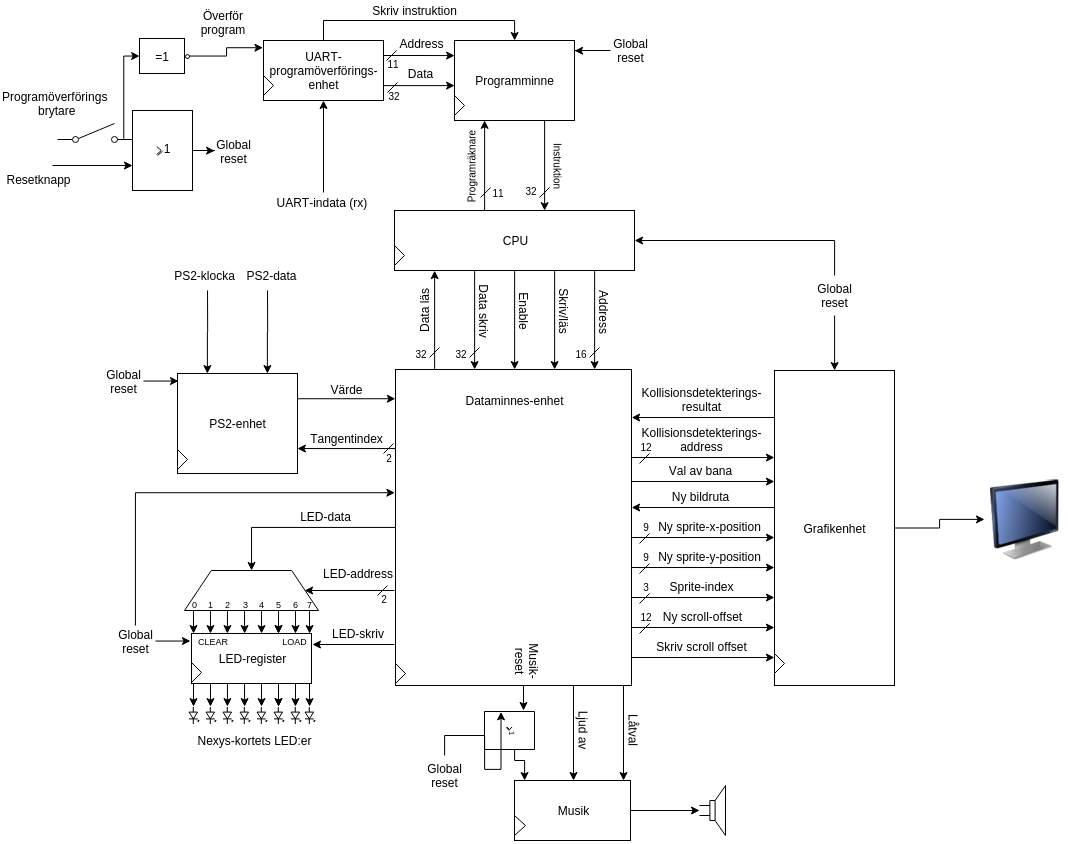
\includegraphics[width=14cm]{../images/overview.png}
	\caption{Översiktligt blockschema\label{overviewscheme}}
\end{figure}

\subsection{CPU}

\begin{figure}[H]
	\centering
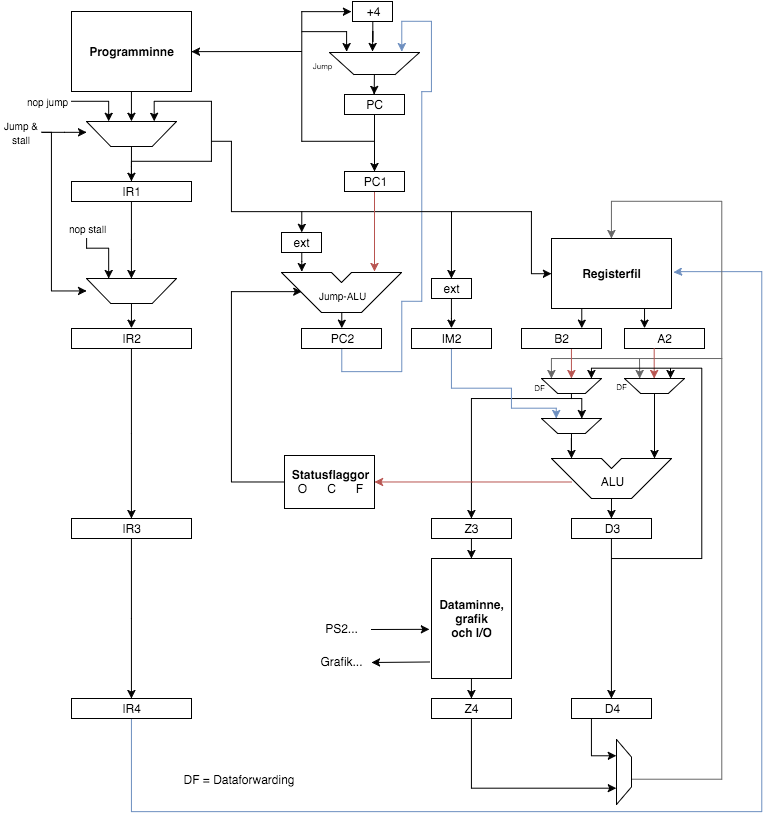
\includegraphics[width=14cm]{../images/CPU.png}
\caption{Blockschema över CPU:n\label{cpuscheme}}
\end{figure}

\subsection{Grafik}

% TODO add graphics

\begin{figure}[H]
	\centering
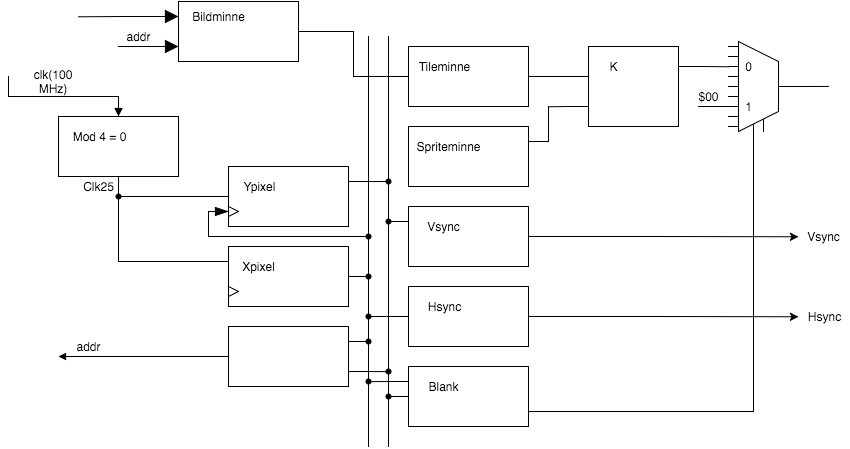
\includegraphics[width=14cm]{../images/vga-schema.png}
	\caption{Blockschema över grafikenheten\label{graphicsscheme}}
\end{figure}

\subsection{Dataminnet och I/O}

Datorn använder minnesmappad I/O för att läsa från tangentbordet och skicka data
till grafik\-enheten.

% TODO elaborate

\subsection{Musik}

Musikmodulen loopar igenom ett speciellt musikminne. Varje element i listan
innehåller tonlängd och tonhöjd. I modulen har man en räknare som räknar ner
tiden för den nuvarande tonen och en annan modul som bara tar in 5 bitar (32
toner $\approx$ 2,5 oktaver) som säger vilken ton som ska spelas just nu. De 5
bitarna används för att slå upp i en tabell över hur långa pulserna ska vara för
den tonen. Sen växlar den bara mellan att skicka ut 0 och 1 på högtalaren.

\begin{figure}[H]
	\centering
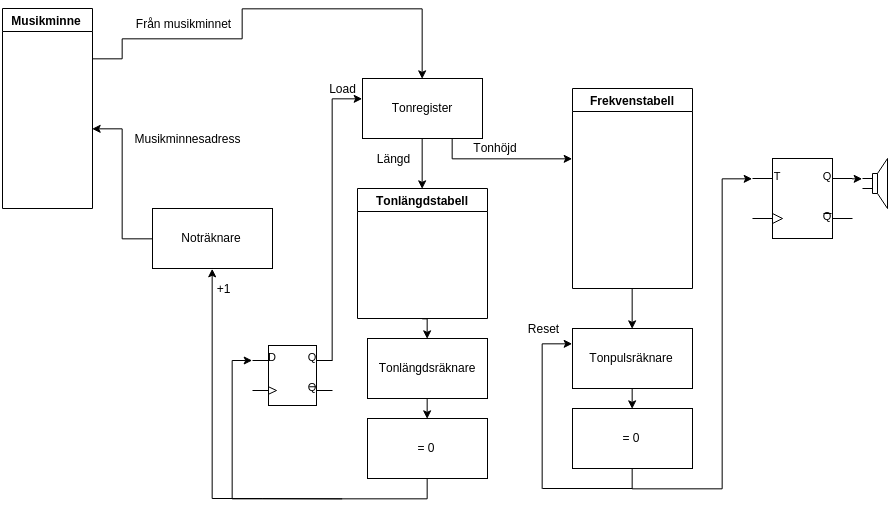
\includegraphics[width=14cm]{../images/Musik.png}
\caption{Blockschema över musikenheten\label{musicscheme}}
\end{figure}

\subsection{Inmatning via PS2}

\begin{figure}[H]
	\centering
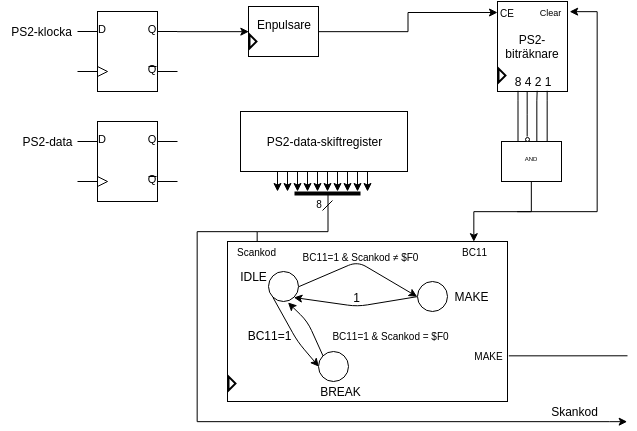
\includegraphics[width=14cm]{../images/PS2.png}
\caption{Blockschema över PS2-enheten\label{ps2scheme}}
\end{figure}

\subsection{Programöverföring via UART}

\begin{figure}[H] 
	\centering
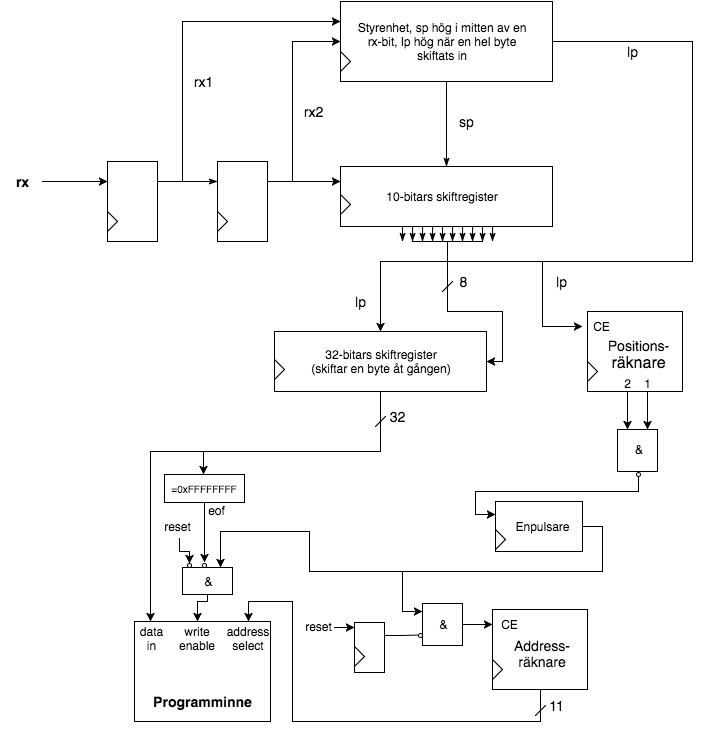
\includegraphics[width=14cm]{../images/UART.png}
	\caption{Blockschema över UART-enheten\label{uartscheme}}
\end{figure}

\section{Mjukvara}

\end{document}
